% !TeX encoding = UTF-8
% !TeX spellcheck = en_US
\section{Required code structure for ECCO}
\IEEEPARstart{E}cco requires a structure similiar to the
file tree shown in figure \ref{fig:overview-2} to be able to parse the product
\\ \ \\
\begin{figure*}[ht]
  \centering
  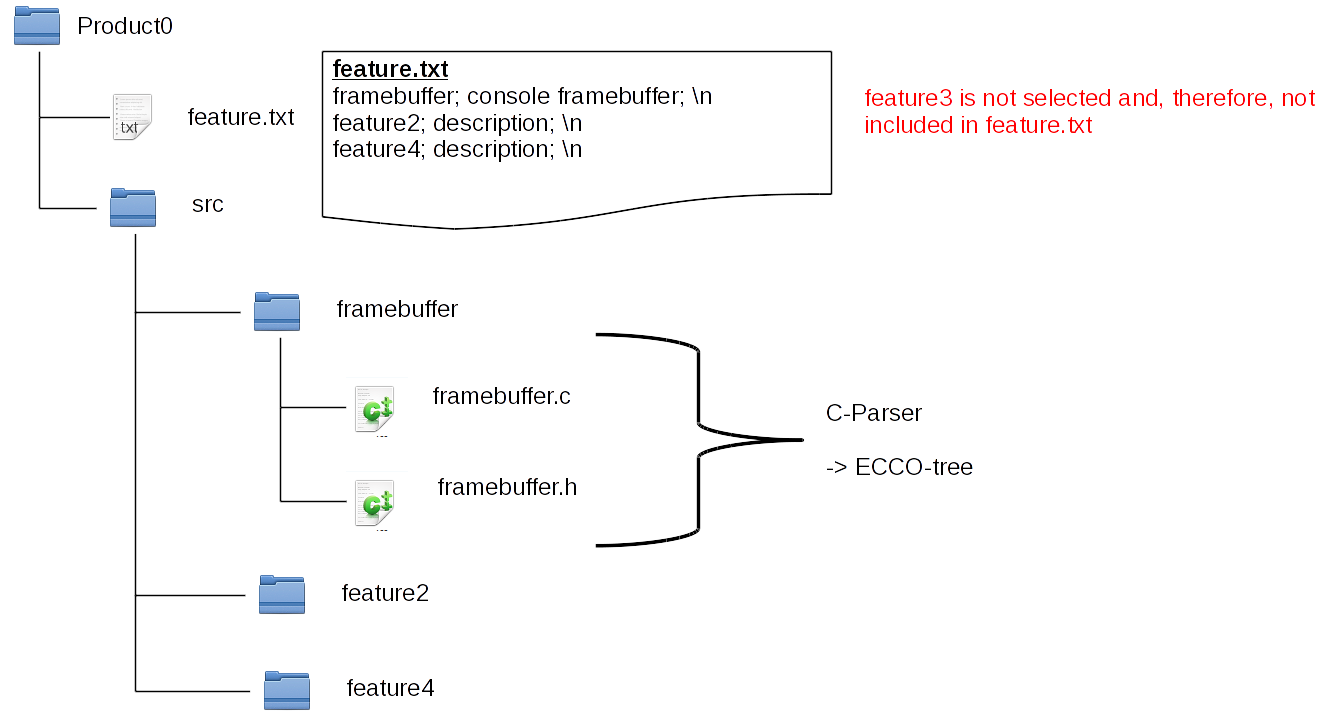
\includegraphics[scale=0.5]{images/overview-2}
  \caption{Overview of required code structure}
  \label{fig:overview-2}
\end{figure*}

The {\it feature.txt} should list all enabled features,
one per line starting with a unique name separated with a semicolon from the feature's description 
and a new-line character at the end.
The file structure should only contain the pruned source code
(so no folders / source files for disabled features). 
The source files should be parsed by some parser and be presented to {\it ECCO} as a tree data structure.

\FloatBarrier
